%\part*{Lezione 03/03/2021}
\section{Modello \textit{a goccia}}
\subsection{La necessità di un nuovo modello}
Torniamo sulle problematiche del modello \textit{a shell}. Prendiamo $\ce{^{130}_{50}Sn_{80}}$: è un pari-pari per cui ci aspettiamo che lo stato fondamentale sia uno $0^+$. I problemi del modello compaiono quando cerchiamo di spiegare lo stato $2^+$ a 1 MeV dal fondamentale. Non ho protoni spaiati perché 50 è un numero magico; per quanto riguarda i neutroni, ne mancano 2 per fare il numero magico 82, allora potremmo provare a promuovere un neutrone da uno dei livelli inferiori. Tuttavia, poiché il salto dev'essere di 1 MeV non può certo venire da $1g_{9/2}$, allora supponiamo inizialmente provenga da $3s_{1/2}$: $5\leq j_{3s} + j_{1h}\leq6$, non portano ad avere un $2^+$. Anche se si prova a cercare un altro stato da cui prendere il neutrone non si riesce a trovarne uno che spieghi $J^\pi=2^+$ e il salto di 1 MeV, poiché è sempre necessario \vir{rompere} una coppia di nucleoni (circa 2 MeV). Inoltre, si osserva la presenza di questo stato (a energie minori) per ogni nucleo pari-pari con circa $150<A<200$, come in Figura \ref{graf2+}.

\begin{figure}[h]
    \centering
    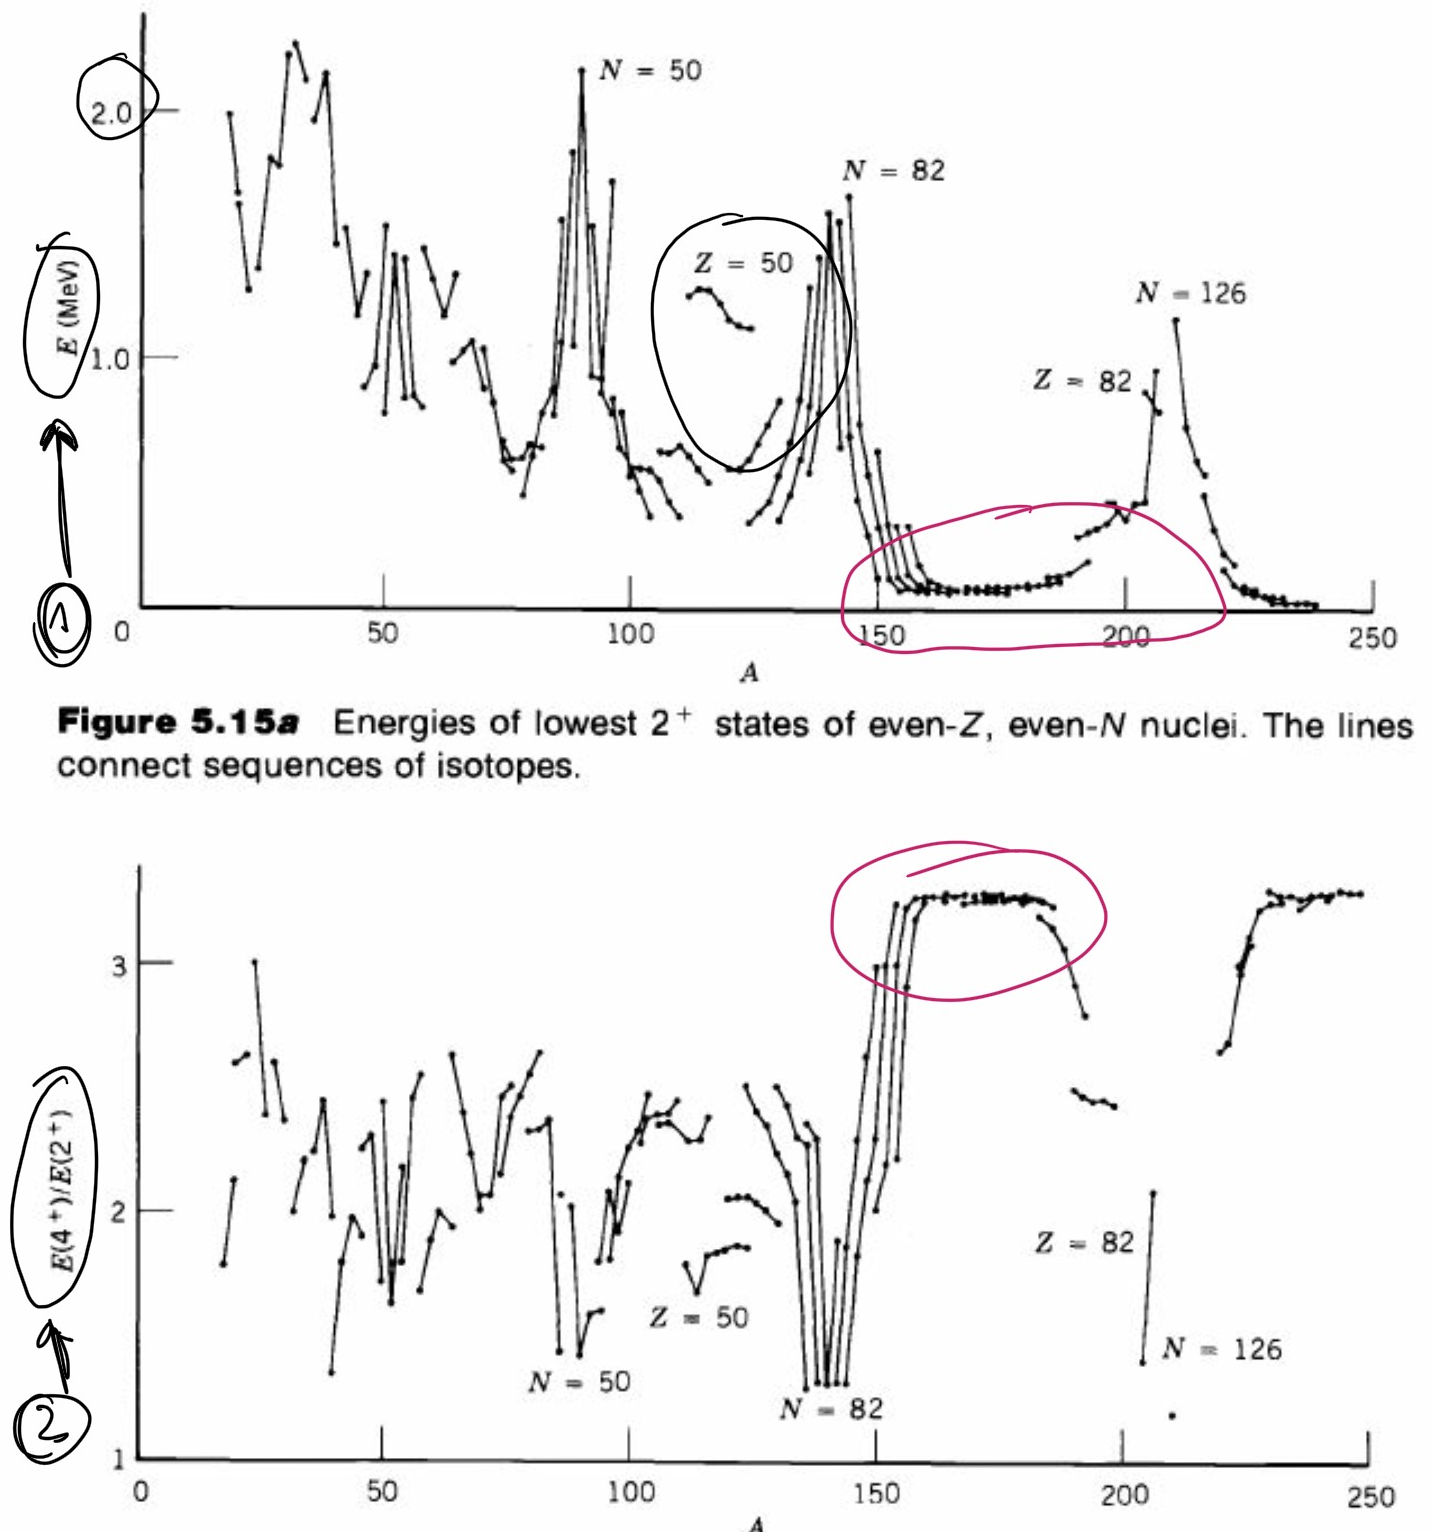
\includegraphics[scale=0.2]{Immagini/150200.png}
    \caption{In basso andamenti del rapporto tra $E(4^+)$ e $E(2^+)$ al variare $A$. Le linee non sono fit, ma collegano semplicemente i dati.}
    \label{graf2+}
\end{figure}
\begin{figure}[h]
    \centering
    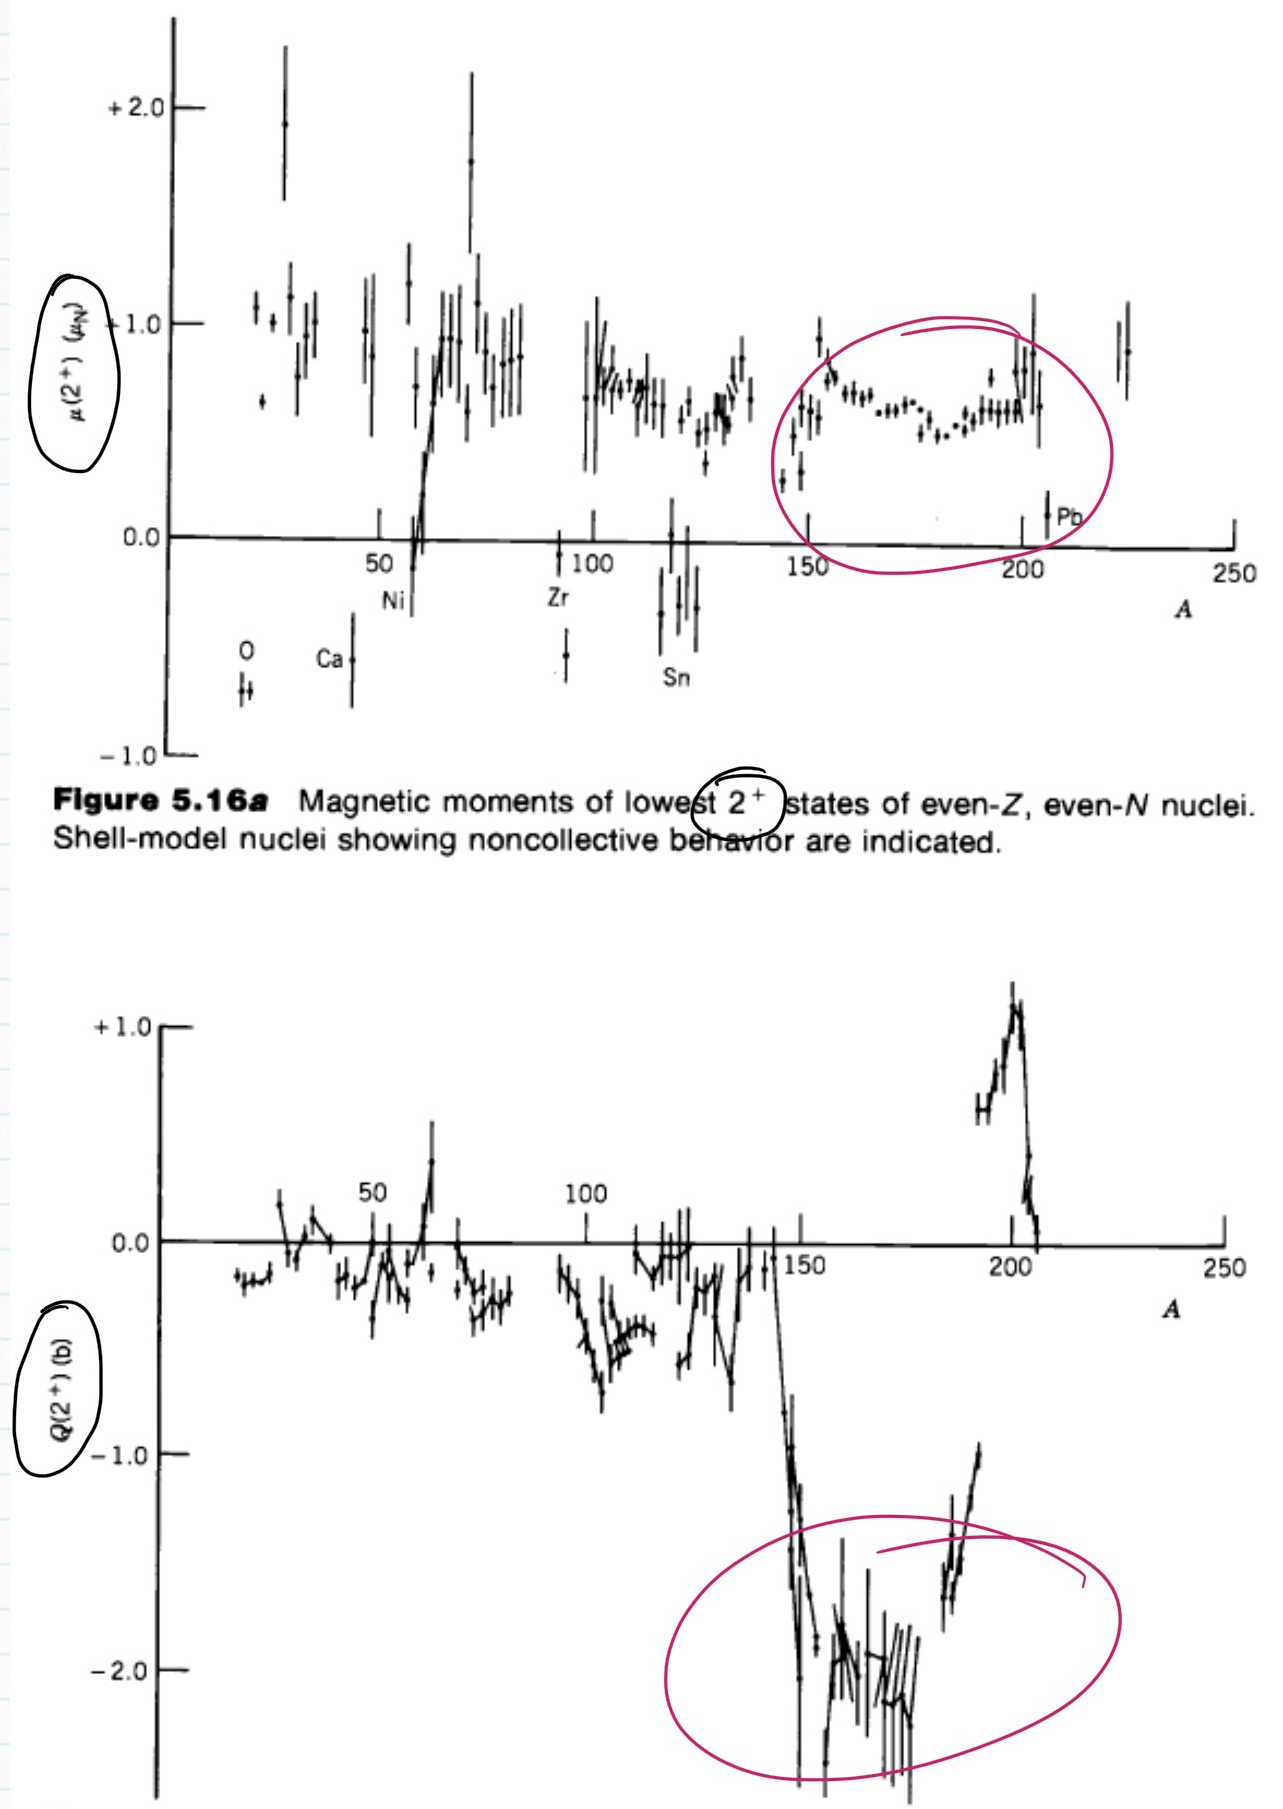
\includegraphics[scale=0.25]{Immagini/150200_2.png}
    \caption{In basso andamento del quadrupolo per lo stato $2^+$ al variare di $A$. Le linee non sono fit, ma collegano semplicemente i dati.}
    \label{graf2+1}
\end{figure}

\subsection{Stati vibrazionali}
Una spiegazione soddisfacente di tali stati eccitati e dell'andamento dei momenti di dipolo magnetico e di quadrupolo elettrico (in Figura \ref{graf2+1}), è data dal \textbf{\textit{Liquid Drop Model}}\index{modelli nucleari! a goccia@\textit{a goccia}}: assunta una configurazione sferica di equilibrio, si descrivono come \vir{vibrazioni} attorno a essa gli stati del nucleo, che a questo punto sono effettivamente stati collettivi (contrariamente al modello \textit{a shell}).\\
Pensiamo allora a una \vir{goccia} sferica che si deforma e definiamo $R(t)$ il raggio in funzione del tempo come:
$$R(t) = R_{av} + \sum_{\lambda\geq 1,\; \mu=-\lambda \dots \lambda}\alpha_{\lambda \mu}(t) \mathcal{Y}_{\lambda\mu}(\theta,\varphi)$$
con simmetria per riflessione $\alpha_{\lambda\mu} = \alpha_{\lambda\,-\mu}$, $\mathcal{Y}_{\lambda\mu}$ l'armonica sferica e $R_{av}=R_0\,A^{1/3}$ (corrispondente a $\lambda = 0$). Per $\lambda=1$ (dipolo) abbiamo una semplice traslazione del centro della sfera (vettore spostamento del $R_{CM}$), quindi non ci interessa; per $\lambda = 2$, invece, si ha $\mathcal{Y}_{2\mu}$ che è legata a un quadrupolo e quindi a una deformazione della struttura. Partendo proprio dal quadrupolo proponiamo una descrizione quantizzata degli stati vibrazionali.

\paragraph{Fononi} Possiamo allora prendere $\lambda=2 $ come unità e definire un quanto di energia vibrazionale, il \textbf{fonone}\index{fonone}, che  in questo caso prenderà il nome di fonone di quadrupolo; quindi $0^+ + $ 1 fonone $\lambda=2$, che si porta dietro $Y_{2\mu}$, $\ell =2$ e $\pi=+$:
$$0^+ + 2^+ = 2^+$$
Il $2^+$ è allora il primo stato eccitato vibrazionale del nucleo, anche se l'energia del fonone in questa trattazione è un parametro libero. Supponiamo allora di aggiungerne un altro: $\mu = \mu_1 + \mu_2$ e $\mu_i = -2, \dots, 2$, da cui $5\cdot 5 = 25$ combinazioni possibili. In realtà non è così, le combinazioni effettive sono solo 15. Guardiamo infatti la Tabella \ref{mumu}: per $\mu=4$ abbiamo una sola possibilità; per $\mu=3$ ne avremmo 2, ma dal momento che il fonone ha \textit{spin} intero la sua funzione d'onda dev'essere simmetrica, di conseguenza le possibilità si riducono a una; per $\mu = 2$ avremmo 3 possibilità, ma si riducono a 2 e così via. 

\begin{table}[!h]
    \centering
    \begin{tabular}{|c|ccccc|}
        \hline
        \multirow{3}{*}{$\mu_2$} & \multicolumn{5}{c|}{$\mu_1$} \\
        \cline{2-6}
         & -2 & -1 & 0 & 1 & 2 \\
        \hline
        -2 & -4 & -3 & -2 & -1 & 0 \\
        -1 & -3 & -2 & -1 & 0 & 1 \\
        0 & -2 & -1 & 0 & 1 & 2 \\
        1 & -1 & 0 & 1 & 2 & 3 \\
        2 & 0 & 1 & 2 & 3 & 4 \\
        \hline
    \end{tabular}
    \caption{Valori di $\mu=\mu_1+\mu_2$ per 2 fononi di quadrupolo.}
    \label{mumu}
\end{table}
\noindent Tenendo conto dello \textit{spin} del fonone, si arriva a 15 combinazioni, che possono essere descritte così:
\begin{displaymath}
\begin{aligned}
&\ell = 4 & &\mu=-4,\dots,4 & &9 \text{ Possibilità} \\
&\ell = 2 & &\mu=-2,\dots,2 & &5 \text{ Possibilità} \\
&\ell = 0 & &\mu=0 & &1 \text{ Possibilità}\\ 
\hline
& & &\text{Tripletto} & &15 \text{ Possibilità} 
\end{aligned}
\end{displaymath}
\noindent Ci aspetteremo dunque un tripletto $0^+,2^+,4^+$ degenere con energia circa il doppio di quella del $2^+$ di un solo fonone. Ci sono evidenze di questo, per esempio, nel $\ce{^{120}_{52}Te_{68}}$\footnote{Detto \textit{\vir{la perfetta goccia vibrante}}.}, dove però compaiono\footnote{Non è stato inserito il disegno dei livelli.}, oltre al $2^+$ e al tripletto, il quintetto $2^+,0^+,3^+,4^+,6^+$ (dovuto a 3 fononi) e il $3^-$ (ovvero un ottupolo $\ell=3$).

\subsection{Bande rotazionali} 
Con il modello vibrazionale abbiamo spiegato gli stati $2^+$ e $4^+$, tuttavia non abbiamo ancora chiarito i problemi per i nuclei con $150<A<200$ per quanto riguarda il loro momento di quadrupolo (molto maggiore rispetto a quello dei nuclei con $A<150$), come in Figura \ref{Q}). \\
Tali valori del momento ci suggeriscono che i nuclei siano fortemente deformati rispetto alla simmetria sferica dello $0^+$, per cui li descriviamo come ellissodi di rotazione:
$$R(\theta,\phi) = R_{av}(1+\beta\, \mathcal{Y}_{20}(\theta,\phi))$$
$$\beta = \frac{4}{3}\sqrt{\frac{\pi}{5}} \frac{\Delta R}{R_{av}}$$
dove $\Delta R$ è la differenza tra semiasse maggiore e minore e (in prima approssimazione) $R_{av}\simeq R_0 A^{\frac{1}{3}}$ è il raggio medio. In base al segno di $\beta$ si ha una figura:
\begin{itemize}
    \item \textbf{prolata}\index{figura!prolata} $\Rightarrow \; \beta >0$, Figura \ref{0303_proobl} a destra.
    \item \textbf{oblata}\index{figura!oblata} $\Rightarrow \; \beta <0$, Figura \ref{0303_proobl} a sinistra.
\end{itemize}
\begin{figure}[h]
    \centering
    \includegraphics[scale=0.7]{Immagini/0303_proobl.png}
    \caption{A sinistra figura oblata, a destra prolata. Questa immagine è stata presa da internet e non fa parte di quelle del corso.}
    \label{0303_proobl}
\end{figure}
Possiamo allora calcolare il momento di quadrupolo magnetico nel sistema di riferimento del nucleo (corotante):
$$Q_0 = \frac{3}{\sqrt{5\pi}}R^2_{av}Z\beta(1+0.16\,\beta)$$
Tuttavia, se una figura prolata ruota può apparire oblata, per cui se il nucleo ha $Q_0>0$ osserviamo un $Q<0$ nel sistema del laboraotorio e questo spiega il valore negativo del momento di quadrupolo. A titolo di esempio, riportiamo il valore per il $2^+$ (per il quale si osserva $Q\sim -2\unit{b}$):
$$-2\unit{b} \simeq Q = -\frac{2}{7} Q_0 \; \Rightarrow \; Q_0 \simeq -7\unit{b}$$
$$\beta \simeq 0.29$$
Abbiamo quindi un nucleo fortemente deformato.\\
\paragraph{Quantizzazione} Per una descrizione quantizzata di tali nuclei scriviamo l'espressione dell'energia cinetica di rotazione:
$$E_{cin} = \frac{1}{2} I \omega^2=\frac{1}{2}\frac{L(L+1)}{I}$$
dove $I=L/\omega$ è il momento di inerzia del nucleo; possiamo allora descrivere\footnote{$\ell = L/\hbar\,\Rightarrow\, E_{cin} = \hbar^2\ell(\ell+1)/2I$.} i loro stati come \textbf{bande rotazionali}\index{bande rotazionali} associate ai livelli energetici:
\begin{displaymath}
\begin{aligned}
\text{St}&\text{ato} & &E_{cin} \\
\hline
&0^+ & &0 \\
&2^+ & 6&\frac{\hbar^2}{2I} \\
&4^+ & 20&\frac{\hbar^2}{2I} \\
&\vdots & \vdots&
\end{aligned}
\end{displaymath}
\begin{figure}[h]
    \centering
    \includegraphics[scale=0.6]{Immagini/0303_liv.png}
    \caption{Livelli energetici dell'afnio.}
    \label{0303_livel}
\end{figure}
\noindent Vediamo come esempio\footnote{L'afnio è importante perché il suo decadimento viene utilizzato in fisica medica.} $\ce{^{176}_{72}Hf_{104}}$, i cui livelli\footnote{Per i calcoli abbiamo usato $\hbar^2/2I \sim 88/6 \sim 14.7$ keV} sono riportati in Figura \ref{0303_livel}:
\begin{displaymath}
\begin{aligned}
E(2^+)&= 6\frac{\hbar^2}{2I}\sim 88\, \mbox{keV} \\
E(4^+)&= 20\frac{\hbar^2}{2I}\sim 293\, \mbox{keV} \\
E(6^+)&= 42\frac{\hbar^2}{2I}\sim 621\, \mbox{keV} \\
E(8^+)&= 72\frac{\hbar^2}{2I}\sim 1064\, \mbox{keV} \\
\Rightarrow \frac{E(4^+)}{E(2^+)}&= 3.33
\end{aligned}
\end{displaymath}
L'ultimo risultato è interessante dal momento che è il valore esatto per i rapporti energetici del $\ce{^{164}_{68}Er_{96}}$. Dunque il modello riproduce con ottimo accordo le osservazioni.

%%%%%%%%%%%%%%%%%%%%%%%%%%%%%%%%%

\chapter{Decadimenti}\label{sec-decadimenti}
In questo capitolo descriveremo in modo rigoroso i decadimenti $\beta$ e $\gamma$\footnote{Per un testo di riferimento sull'argomento vedi \complrif{compl-krane}.}. Il capitolo copre le lezioni 03/03/2021, 04/03/2021, 08/03/2021 e 10/03/2021
\section{Decadimento $\beta$}
Esistono tre tipologie di \textbf{decadimento} $\beta$:
\begin{itemize}
    \item $\beta^-$: decadimento di un neutrone.
    \item $\beta^+$: decadimento di un protone.
    \item $\varepsilon$: cattura elettronica da parte di un protone.
\end{itemize}
\noindent Abbiamo quindi:
\begin{displaymath}
\begin{aligned}
&\beta^- & \ce{^A_ZX_N}&\to \ce{^A_{Z+1}Y_{N-1}} + e^- + \bar{\nu}_e & n&\to p + e^- + \bar{\nu}_e \\
&\beta^+ & \ce{^A_ZX_N}&\to \ce{^A_{Z-1}Y_{N+1}} + e^+ + \nu_e & p &\to n + e^+ + \nu_e \\
&\varepsilon & \ce{^A_ZX_N} + e^-&\to \ce{^A_{Z-1}Y_{N+1}}  + \nu_e & p+e^- &\to n + \nu_e
\end{aligned}
\end{displaymath}
dove abbiamo separato i processi nucleari da quelli base (che avvengono nel nucleo). Per capire se questi sono\footnote{Con \textit{permessi} e \textit{proibiti} si intende rispettivamente \vir{probabili} e \vir{poco probabili}.} \textit{permessi} o \textit{proibiti} è necessario calcolare il $Q$-\textit{value} $Q=\sum T_i$; possiamo momentaneamente approssimare $m_{\nu}\simeq 0$ MeV e $m_e \simeq 0.5$ MeV, ma dobbiamo considerare $m_n \not \simeq m_p$ per cui $m_n - m_p \simeq 1.3$ MeV: si osserva immediatamente che $m_n>m_p$ implica $\beta^-$ \textit{permesso} ($Q>0$) e $\beta^+$ \textit{proibito} ($Q<0$). Dunque, il protone se libero non decade\footnote{Anche in questo caso si intende che i tempi di decadimento sono \vir{lunghissimi}.}, ma può fare $\beta^+$ solo se è legato e l'energia di legame sia almeno 1.3 MeV.

\subsection{La questione dei neutrini} 
Fino al 1931, anno in cui Pauli propose l'esistenza del neutrino, i risultati dello spettro elettronico del decadimento $\beta$ furono motivo di intensa discussione: trascurando la presenza di una terza particella nei prodotti, ci si aspetterebbe un andamento del numero di elettroni in funzione dell'energia cinetica degli stessi di tipo a $\delta$, centrata sul valore del $Q$-\textit{value}\footnote{dalla conservazione dell'energia si ha appunto $m(X) = m(Y) + m_e + T_e$ per cui $Q\simeq T_e$}.
Tuttavia, quello che invece si osserva è un andamento continuo decrescente come quello riportato in Figura \ref{0303_ne}.
\begin{figure}[h]
    \centering
    \includegraphics[scale=0.5]{Immagini/0303_nume.png}
    \caption{Distribuzione del numero di neutrini in funzione dell'energia cinetica.}
    \label{0303_ne}
\end{figure}
Inizialmente, si diede come spiegazione a questo fatto la possibilità che gli elettroni prima di uscire dal campione urtassero contro altri elettroni atomici, ridistribuendo così la loro energia cinetica, ma non era esaustiva. Fu Pauli a risolvere la questione, ipotizzando per primo l'esistenza di un'altra particella non rivelata (che appunto Fermi nel 1934 chiamò \textit{neutrino}).\\ Dal calcolo del $Q$-\textit{value}:
$$Q = m_n - m_p - m_e - m_\nu \simeq 0.78 \;\mbox{MeV} - m_\nu$$
La misura di questo dà, quindi, una stima della massa del neutrino. Il problema è che è estremamente difficile da fare: i dati riportarono $Q = (0.782 \pm 0.013)$ per cui $m_\nu \simeq 0$ entro 13 keV\footnote{Con le misure più recenti si ha $m_\nu \simeq 0$ entro 1 eV}. Dunque, non è una \vir{cattiva} approssimazione quella di trascurare la massa del neutrino rispetto alle altre masse in gioco, a meno che i neutrini non siano i \vir{protagonisti} del fenomeno in esame\footnote{Vedremo in seguito un esempio in cui questo avviene.}. 
\paragraph{Q-value}\label{sec-qvalue}
Calcoliamo dunque il $Q$-\textit{value} di questi decadimenti\footnote{Procederemo in realtà al calcolo esplicito solo del decadimento $\beta^-$, poiché gli altri sono concettualmente identici.} trascurando la massa del neutrino. Definiamo la massa atomica come:
$$m_{at} (\ce{_{Z}X}) \equiv m(\ce{^A_ZX_N})+Zm_e - \sum_{i=1}^Z B_i$$
dove $B_i$ è l'energia di legame dell'$i$-esimo elettrone.
\begin{displaymath}
\begin{aligned}
Q_{\beta^-} &= m_{at}(\ce{_ZX}) - Zm_e + \sum_{i=1}^Z B_i - m_{at}(\ce{_{Z+1}Y}) + (Z+1) m_e - \sum_{i=1}^{Z+1} B_i - m_e= \\
&= m_{at}(\ce{_ZX}) - m_{at}(\ce{_{Z+1}Y}) + \sum_{i=1}^Z B_i - \sum_{i=1}^{Z+1} B_i \simeq \\
&\simeq m_{at}(\ce{_ZX}) - m_{at}(\ce{_{Z+1}Y}) \\
Q_{\beta^+} &= m_{at}(\ce{_ZX}) - m_{at}(\ce{_{Z+1}Y}) - 2m_e \\
Q_{\varepsilon} &= m_{at}(\ce{_ZX}) - m_{at}(\ce{_{Z+1}Y}) - B_n
\end{aligned}
\end{displaymath}
dove abbiamo fatto l'approssimazione $Z\sim Z+1$ poiché stiamo considerando atomi con $Z$ molto \vir{alto} e dove abbiamo definito $B_n$ la \textit{binding energy} per l'elettrone catturato dell'$n$-esimo shell\footnote{Per qualche dettaglio vedi \complrif{compl-epsilon}.} ($n = k,L,\dots$). Vediamo alcuni esempi:
\begin{displaymath}
\begin{aligned}
&\text{Decadimento} & &Q & \tau_{\frac{1}{2}}& \\
\hline
&\ce{^{23}Ne} \betamin \ce{^{23}Na} & &4.38 & 38&\,\mbox{s} \\
&\ce{^{99}Tc} \betamin \ce{^{99}Ru} & &0.29 & 2\cdot 10^5&\,\mbox{y} \\
&\ce{^{25}Al} \betaplu \ce{^{25}Mg} & &3.26 & 7.2&\,\mbox{s} \\
&\ce{^{134}I} \betaplu \ce{^{134}Te} & &2.14 & 4.2&\,\mbox{d} \\
\end{aligned}
\end{displaymath}
Dai dati sembra che non vi sia correlazione tra il $Q$-\textit{value} e il periodo di dimezzamento, che copre vari ordini di grandezza.\\
Fermi riuscì a darne una spiegazione costruendo una teoria per il decadimento.